\documentclass[12pt]{article}

\usepackage[margin=1.5in]{geometry}
\usepackage{amsmath}
\usepackage{amsthm}
\usepackage{amssymb}
\usepackage{graphicx}
\usepackage{verbatim}
\usepackage{fullpage}
\usepackage{psfrag}
\usepackage{url}

\usepackage[small,bf]{caption}

\setlength{\captionmargin}{30pt}

\input defs.tex
\newcommand{\sign}{\mathop{\bf sign}}

\bibliographystyle{alpha}

\title{Symbolic Subdifferentiation in Python}
\author{Maurizio Cal\'o and Jaehyun Park\\
EE 364B Project Final Report\\
Stanford University, Spring 2010-11}

\begin{document}
\maketitle

\section{Introduction}
\subsection{Subgradient-PY}
We implemented a Python package \verb'Subgradient-PY' (\verb'spy') that solves
optimization problems using subgradient methods. Below are some features of \verb'spy'.
\begin{itemize}
\item The objective function and constraints need not be differentiable.
\item Due to little space usage, \verb'spy' can be used to solve large problems.
\item \verb'spy' can be combined with primal or dual decomposition techniques to develop distributed algorithms.
\end{itemize}

\subsection{Motivation}
This project is motivated by the first two weeks of EE 364B lectures on subgradients and subgradient methods. Also, somewhat unexpectedly, there is yet no software package that can automatically compute subgradients of convex functions, or implement subgradient methods. (S. Boyd, personal communication, April 2011)

\verb'spy' is implemented in Python. The objected-oriented paradigm of Python made it easy to implement a nontrivial project in a short time, without worrying too much about technical details. There has been some attempts to model convex optimization problems in Python, such as \verb'cvxpy', \verb'cvxmod', and \verb'cvxopt'. However, rather than integrating our project with these existing softwares, we decided to implement everything from scratch, for educational purposes.

\section{A Quick Start}
\verb'spy' can be downloaded from \url{http://www.stanford.edu/~liszt90/spy}. There is no installation package, so one can simply download the codes and unzip it to a directory named \verb'spy'.

\subsection{Example Code}
The following code solves a simple convex optimization problem using \verb'spy'.

\begin{quote}
\begin{verbatim}
from spy import *
x = var('x')
y = var('y')
ex = max(x + y, 2 * x - y) + square(x)
constraints = [geq(x, y), leq(norm2([x, y]), 1)]
prob = minimize(ex, constraints)
(optval, optpoint) = prob.solve()
\end{verbatim}
\end{quote}

\noindent Let us examine the code line by line:

\begin{itemize}
\item Line 1: Import all modules from the \verb'spy' package.
\item Line 2-3: Declare $x$ and $y$ as (scalar) optimization variables.
\item Line 4: Form an instance of the Expression class, corresponding to the mathematical expression: $\max(x+y,2x-y)+x^2$.
\item Line 5: Specify the constraints of the optimization problem: $x \geq y$ and $\sqrt{x^2+y^2} \leq 1$.
\item Line 6: Define the optimization problem: ``minimize \verb'ex' subject to \verb'constraints'.''
\item Line 7: Solve the optimization problem using a subgradient method.
\end{itemize}

\noindent Printing out \verb'optval' and \verb'optpoint' gives the following:

\begin{quote}
\begin{verbatim}
-0.250040107722
{'y': -0.50654454816398864, 'x': -0.50662859414656536}
\end{verbatim}
\end{quote}

\noindent The analytic solution is $x=y=-1/2$ with the optimal value $f^\star = -1/4$.

\section{Basics}

\subsection{Main Classes}
\verb'spy' implements three important classes:

\begin{itemize}
\item Expression: Any real-valued mathematical expression is an object
of Expression type. It can contain variables whose values are not
predetermined. For convex expressions, subgradients can be evaluated at a given point.
\item Constraint: A constraint is an inequality of the form
$(\mbox{convex}) \le (\mbox{concave})$ or an equality of the form
$(\mbox{affine}) = (\mbox{affine})$.
\item (Optimization) Problem: A problem is a triplet of the form (minimize/maximize, objective, list of constraints).
\end{itemize}

\noindent The essential part of the project is to compute subgradients correctly
and efficiently, since all other methods rely heavily on subgradients.

\subsection{Declaring Variables}
One can declare a variable using the following command.

\begin{quote}
\begin{verbatim}
x = var('x')
\end{verbatim}
\end{quote}

\noindent The meaning should be clear from the syntax; the line above declares a
variable whose name is \verb'x' without a value assigned to it. The object \verb'x' is a symbolic link to the variable with the identifier string \verb,'x',. This allows users to recover variables from identifier strings even if they lose variable objects.

\subsection{Forming an Expression}
With variables, it is possible to form more complicated expressions. To
provide a clean interface to the user, we have overloaded basic arithmetic operators as
well as some of the Python built-in functions. This allows users to form
expressions in a natural way. For instance, the following line will create an expression named \verb'ex'.

\begin{quote}
\begin{verbatim}
ex = abs(x - 3) + exp(x)
\end{verbatim}
\end{quote}

\noindent The expression above corresponds to a mathematical expression
$|x-3|+e^x$. It should be noted that \verb'spy' does not attempt to
simplify a given expression, nor does it immediately compute the value of
a newly formed expressions. All computations are done lazily; the
values will be computed only when the \verb'get_value' method is called on
it. Internally, the expression is stored as a tree shown in the following diagram:

\begin{center}
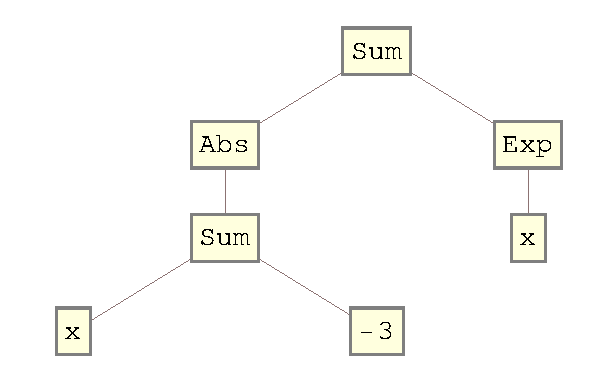
\includegraphics[width=0.45\textwidth]{expr}
\end{center}

\subsection{Retrieving Values or Subgradients}
Because the values of variables in an expression is not predetermined, a user needs to specify them manually in order to retrieve the actual value or a subgradient of the expression. The values of the variables are not passed in as a list of numbers as one might expect. Rather, the values are passed as a dictionary that maps the name of variables to their values. The benefit of this design is that one can readily access the value of a variable by its name.

\begin{quote}
\begin{verbatim}
varmap = {'x': 1.5, 'y': -2}
val = ex.get_value(varmap)
g = ex.subgrad(varmap)
\end{verbatim}
\end{quote}

\noindent The code above will evaluate the expression \verb'ex' at $x=1.5$ and $y=-2$, and store the (scalar-valued) result in \verb'val'. Note that the argument to the \verb'get_value' method is a dictionary, not a list of coordinates. The next line computes a subgradient of \verb'ex' evaluated at the same point, storing the result into \verb'g'. The data type of \verb'g' is the same as that of \verb'varmap'. For these methods to work correctly, users need to specify the values of all the variables present in the expression. Otherwise, \verb'nan' will be returned. Users can retrieve all the variables in an expression by calling \verb'get_vars' method on it.

The subgradient computation, as mentioned above, is the most crucial part of this project. This feature has been tested by multiple scripts that solve simple optimization problems. Also, whenever a new library function is added, a unit test is implemented in order to ensure that the functions behave as expected.

\subsection{Specifying Constraints}
One can use \verb'leq', \verb'eq', or \verb'geq' to construct a constraint
object. At construction time, \verb'spy' automatically checks whether inequalities
and equalities follow the DCP ruleset. Constraints should be of the form
$(\mbox{convex}) \le (\mbox{concave})$ or 
$(\mbox{affine}) = (\mbox{affine})$.

Another important feature of the Constraint class is the \verb'cutting_plane'
function. This method returns a deep cutting plane whenever a constraint is
violated. Let $f(x) \le 0$ be a constraint. From the definition of subgradients, $f(z) \ge f(x)+g^T(z-x)$ holds for all $z$, where $g \in \partial f(x)$. If $f(x)>0$, then for $f(z)\le 0$ to hold, we need $g^T z + f(x)-g^T x<0$.


\subsection{Solving Optimization Problems}
One can solve convex optimization problems using the following syntax:

\begin{quote}
\begin{verbatim}
myprob = minimize(ex, [cons1, cons2])
(optval, optpoint) = myprob.solve()
\end{verbatim}
\end{quote}

\noindent The lines above minimizes the expression \verb'ex' subject to two constraints
\verb'cons1' and \verb'cons2' using the subgradient method. As a result,
the optimal point as well as the objective value at that point will be
returned. Advanced users can specify the step size rule used by the
method.

\section{Technical Details}

\subsection{Computation of Subgradients}
Subgradient computations are done recursively, and the procedure is
analogous to the chain rule for differentiable functions. 
For each library function, we've implemented a method that computes 
its subgradient at a given point. For the complete list of library functions, see section \ref{libfunctions}.

Subgradients of more complicated expressions can be computed 
using the composition rule \cite{subg}:
\begin{itemize}
\item Let $f(x) = h(f_1(x), \ldots, f_k(x))$ with $h$ convex non-decreasing,
  $f_i$ convex.
\item Find $c \in \partial h(f_1(x), \ldots, f_k(x))$,  $g_i \in \partial
  f_i(x)$
\item Then, $g = c_1 g_1 + c_2 g_2 + \cdots + c_k g_k$ is a subgradient of $f$ at $x$.
\end{itemize}


\subsection{DCP ruleset}
Whenever a constraint is specified, the constraints class automatically checks whether inequalities and equalities follow the DCP ruleset \cite{guide}. Similarly, the problem class checks whether the objective of the minimization (resp. maximization) is convex (resp. concave). This is done by applying the general vector composition rule \cite{cvx}, using the monotonicity and convexity properties of the atomic functions.


\subsection{Subgradient Method}
The \verb'solve' method of the Problem class implements a subgradient method, which is similar to gradient descent methods for minimizing differentiable functions. Consider the following optimization problem.

\begin{equation*}
\begin{aligned}
&\mbox{minimize}&&f(x)\\
&\mbox{subject to}&&f_i(x) \le 0, \quad i = 1, \ldots, m.
\end{aligned}
\end{equation*}

By default, the \verb'solve' method sets every variable in $f$ as zero, and repeatedly applies the following update rule.

\begin{itemize}
\item Let $x^{(k)}$ be the $k$th iteration point. If $x^{(k)}$ is feasible, find $g^{(k)} \in \partial f(x^{(k)})$. Otherwise, find the constraint that is most violated, say $f_i$, and find $g^{(k)} \in \partial f_i(x^{(k)})$.
\item Set the next point as $x^{(k+1)}:=x^{(k)}-\alpha_k g^{(k)}$, where $\alpha_k$ is $k$th step size.
\end{itemize}

If the step size rule is not specified, \verb'spy' uses $\alpha_k = 1/k$ as the default step size. Custom step size rules can be used as well, using a syntax like the following:

\begin{quote}
\begin{verbatim}
stepsize = (var('f') - f_estimate) / square(var('gnorm'))
prob.solve(stepsize)
\end{verbatim}
\end{quote}

\noindent The argument that is passed to the \verb'solve' method can be any expression of three variables, \verb'f', \verb'gnorm', and \verb'iter', which correspond to $f^{(k)}$, $\left\|g^{(k)}\right\|_2$, and $k$, respectively. The step size must evaluate to a positive number during the execution of the \verb'solve' method.

Finally, one can specify the initial point $x^{(1)}$ as an additional argument to \verb'solve'. In this case, the step size rule must be provided as well.

\subsection{Library Functions}
\label{libfunctions}
The following list contains the functions that are implemented in the current version of \verb'spy'. For more details, please refer to the \verb'cvx' user guide \cite{guide}.
\begin{itemize}
\item \verb'abs', \verb'max', \verb'min', \verb'pos', \verb'power', \verb'power_pos'
\item \verb'exp', \verb'log', \verb'log_sum_exp', \verb'rel_entr'
\item \verb'norm1', \verb'norm2', \verb'berhu', \verb'huber'
\item \verb'square', \verb'square_pos', \verb'sqrt', \verb'geo_mean', \verb'quad_over_lin'
\end{itemize}

\section{Limitations}
We are aware of the following issues with \verb'spy'.
\begin{itemize}
\item \verb'spy' does not work well with equality constraints (yet).
\item Convergence behavior depends on the step sizes, so it is up to users to give a ``right'' step size rule.
\item Currently, \verb'spy' cannot detect if the given problem is unbounded.
\item \verb'spy' only works with scalar-valued variables and expressions. We have a simple implementation of the matrix class, but it is not yet integrated with \verb'spy'.
\end{itemize}


\begin{thebibliography}{99}
\bibitem{subg} S. Boyd, \emph{Subgradients}, EE 364B Lecture Slides, 2011.
\bibitem{guide} M. Grant and S. Boyd, \verb'cvx' \emph{Users' Guide}, 2011.
\bibitem{cvx} S. Boyd, \emph{Convex Functions}, EE 364A Lecture Slides, 2011.
\end{thebibliography}

\end{document}

